\documentclass[conference]{IEEEtran}
\IEEEoverridecommandlockouts
% The preceding line is only needed to identify funding in the first footnote. If that is unneeded, please comment it out.
\usepackage{cite}
\usepackage{amsmath,amssymb,amsfonts}
\usepackage{algorithmic}
\usepackage{graphicx}
\usepackage{textcomp}
\usepackage{xcolor}
\def\BibTeX{{\rm B\kern-.05em{\sc i\kern-.025em b}\kern-.08em
    T\kern-.1667em\lower.7ex\hbox{E}\kern-.125emX}}
\begin{document}

\title{Cyberbullying Auto Detection\\}

\author{\IEEEauthorblockN{Wenqu Wang}
\IEEEauthorblockA{\textit{School of Information} \\
\textit{University of California, Berkeley}\\
Berkeley, CA, USA \\
jackw@ischool.berkeley.edu}
\and
\IEEEauthorblockN{Casey Yoon}
\IEEEauthorblockA{\textit{School of Information} \\
\textit{University of California, Berkeley}\\
Berkeley, CA, USA \\
caseyhyoon@ischool.berkeley.edu}
}

\maketitle

\begin{abstract}
Cyberbullying has had an immense impact on mental health for its victims on social media platforms. For these victims, creating a system to address/prevent these negative encounters would help create a more positive community. This project explored the use of neural networks and feature extraction techniques to classify sentiment on Twitter data.
\end{abstract}

\begin{IEEEkeywords}
Machine Learning, Natural Language Processing
\end{IEEEkeywords}

\section{Introduction}
The development of mobile internet has made it possible for social media platforms, like Twitter and YouTube, to amass such popularity and have largely altered people’s lifestyles by providing users with a new way of communication that is free, convenient, and entertaining. However, these platforms have also given way to cyberbullying, a new form of electronic violence characterized by its lack of retribution for its perpetrators and whose victims range from normal personnel to celebrities or popular influencers/bloggers. Cyberbullying has had an immense impact on mental health for its victims, many of whom suffer depression and anxiety; as a result, suicide has become an unfortunate consequence due to the mental and even physical reactions from cyberbullying.

The challenges to this problem, like most sentiment analysis problems, are the fluidity of language and the context in which cyberbullying comments are posted. This context includes the target of said cyberbullying and topic of conversation. In this project, we will utilize and compare several algorithms to find the highest classification accuracies on datasets from Twitter. By applying natural language processing (NLP) techniques, cyberbullying comments can be detected, screened/blocked in the hopes of creating less hostile online communities. 


\section{Overview}

\subsection{Background}

Cyberbullying is becoming a serious problem as the rapid growth in the number of internet users. There are about 4.66 billion internet users all over the world today, and this number grew by 319 million in the past 12 months. With the vast amount of users online, it is very difficult to control the violent practices. Fortunately, the growth of techniques related to natural language processing provides a potential solution, which is efficient and accurate, to the problem of cyberbullying. By analyzing the user sentiment using algorithms, the cyberbullying comments could be detected and further blocked by the server.

In the rest of this section, the authors will discuss approaches to solve this problem using NLP.

\subsection{Dataset}

The authors initially explored Cyberbullying Datasets from Mendeley Data, which contains labeled user comments data collected from various platforms like Kaggle, Twitter, and Youtube. We chose the following three datasets for sentiment analysis on Twitter:

\begin{center}
Twitter\_parsed\_dataset.csv

Twitter\_racism\_parsed\_dataset.csv

Twitter\_sexism\_parsed\_dataset.csv
\end{center}

The authors are interested in tweets that identify to be racist or sexist -- these negative traits go against community guidelines and are the focus of our classification. Merging all three datasets together, the dataset has 45197 entries. 10694 (23.67\%)  of these entries are neutral, while the other 34503 (76.33\%) tweets have been labeled either racist or sexist.

\subsection{Sample Tweets}
\begin{quotation}
\emph{RT @Mooseoftorment Call me sexist, but when I go to an auto place, I'd rather talk to a guy.}
\end{quotation}
\begin{quotation}
\emph{A good Muslim is good despite his bad religion, not because of it.}
\end{quotation}
\begin{quotation}
\emph{@DianH4 Islam doesn't answer anything.  It pretends to answer with illogical and delusional superstition.}
\end{quotation}

The above messages contains sexism or racism content and is marked positive in the dataset.

\begin{quotation}
\emph{Woo can't wait to see what happens!!! \#mkr}
\end{quotation}
\begin{quotation}
\emph{@halalflaws @biebervalue @greenlinerzjm I read them in context.No change in meaning. The history of Islamic slavery.}
\end{quotation}
\begin{quotation}
\emph{@OneLegSandpiper @DblBlackDs Show me some pictures of them beheading people and reinstating slavery. Leftist moral equivalents are stupid.}
\end{quotation}

These messages are examples of non-bullying tweets. Noticed that some of these tweets also contain bad sentiment or racist keywords, but the main focus of the tweet is not to bully someone.

\subsection{Data Cleaning }

The authors were given raw tweets like the samples shown in the previous section. As noticed,  tweets can contain a lot of handles (@), hashtags (\#), and retweet labels (RT). The fluidity of language present in twitter data prompted a bit of consideration before tokenization:

\begin{itemize}
\item Addressing Twitter handles (@user) and retweet labels (RT)

\item Removal of punctuation, numbers and special characters

\item Lowercasing
\end{itemize}

Additionally, the authors did not remove hashtags and retweet labels (RT). Including hashtags into the vocabulary can make sure not to take away unique sentiment values related to certain hashtags and  retweet labels are not removed as they are superficial. Once the tweets are cleaned, they are split up into tokens to prepare for featurization.


\subsection{Word Embeddings}

In order to train classification models, our preprocessed data need to be converted to features. Tf-idf vectorization, which accounts for word frequencies, will be used as our baseline featurization method. Counting the number of times a certain token appears in a corpus is a simple plan for us to identify relationships between frequencies and text sentiment; however, nothing more.

	Several existing research papers have proposed use of Word2Vec word embeddings in future research to initialize classification models, specifically convolutional neural networks. [1](Huang, Qianjia, et al.) Word2Vec, as a shallow neural network used to obtain word vectors, better represents our tokenized tweets as it utilizes word context. 

	Finally, Bidirectional Encoder Representations from Transformers (BERT) was another pre-trained processing model that piqued our interest because it was a higher level tokenizer that maintained sequence information.



\section{Models}
A lot of existing machine learning algorithms and models can be applied to the problem of cyberbullying auto detection. The authors focus specifically on the performance of the combinations of different word embeddings and model. In this section, the authors will explain four of the models: Baseline Model, Tf-idf with Feed-Forward Neural Network, Word2Vec with Convolutional Neural Network, and BERT.

\subsection{Baseline Model}
The authors built our baseline classification model using one-class classification with an accuracy of 0.76, that is, if we simply classified a tweet to be racist or sexist, we’d be correct about 76\% of the time. For our subsequent models, any accuracy score lower than this baseline will not be considered as results would be worse than random guessing.

	We also decided to use our baseline Tf-idf word embeddings with a logistic regression model as another baseline comparison as we introduce alternative models and also word embeddings that hopefully capture significantly better results. We achieve an accuracy of about 85\% with this baseline.


\subsection{Tf-idf with Feed-Forward Neural Network}
By training a 2-hidden-layer feed-forward neural network with Tf-idf embedded data, the model achieved an accuracy of 94.8\%. In order to handle the input dimension for neural networks, authors decided to use 500 hundred as the max number of features of Tf-idf so that each input has 500 features. After the input layer, the data is then passed to two hidden layers with ReLU activation. Finally, a sigmoid layer will map the hidden layer output into a number between zero and one so that the final output could be determined.

The training process takes about one second to run for each epoch, which is pretty efficient.

\begin{figure}[htbp]
\centerline{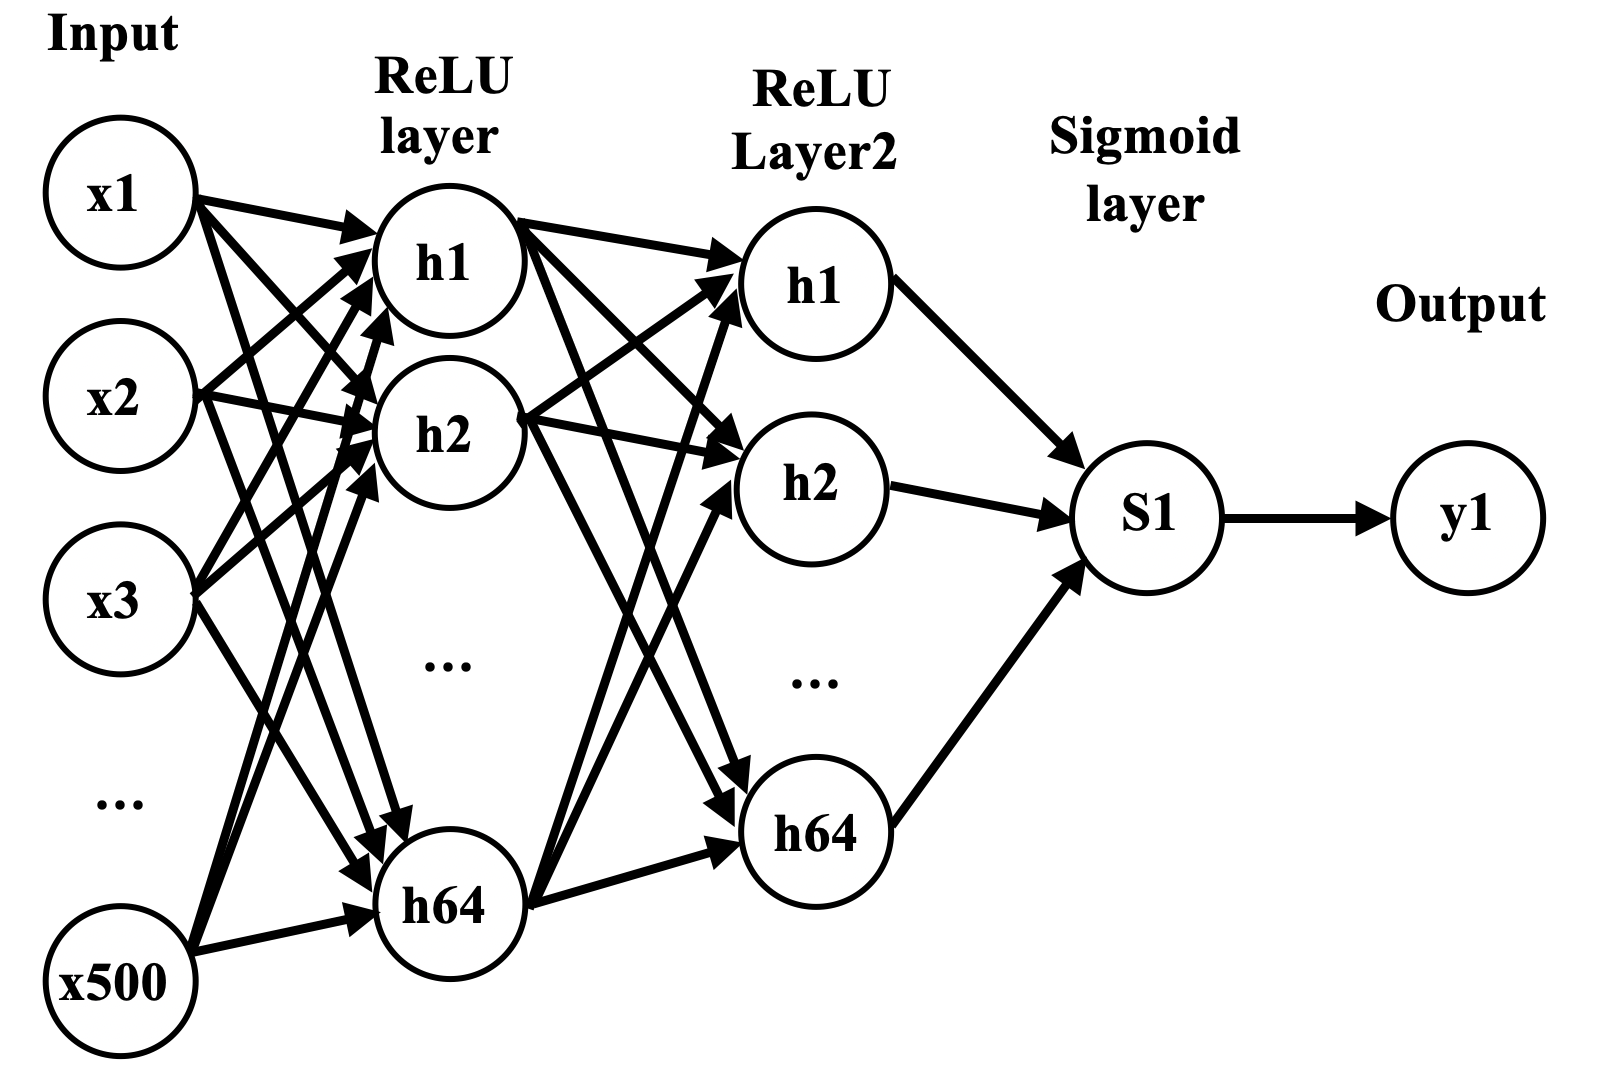
\includegraphics[width=70mm]{fig1.png}}
\caption{Feed-Forward Neural Network Architecture}
\label{fig}
\end{figure}

\subsection{Word2Vec with Convolutional Neural Network (CNN)}

Entering the tokenized tweets into a size-200 word2vec, the model generated a vocabulary of size 19645, which is approximately 20000. As a result, a 10000 * 200 embedding matrix is built and will be put into CNN as the embedding layer. After the embedding layer, the word vectors are then passed into a layer of 1D convolution and another max-pooling layer, and finally the fully connected layers.

Under such architecture, the model achieved accuracy of 98.04\%, which improved significantly compared to the previous model. As for efficiency, each batch takes about 83 seconds to train, which is fairly efficient.

\begin{figure}[htbp]
\centerline{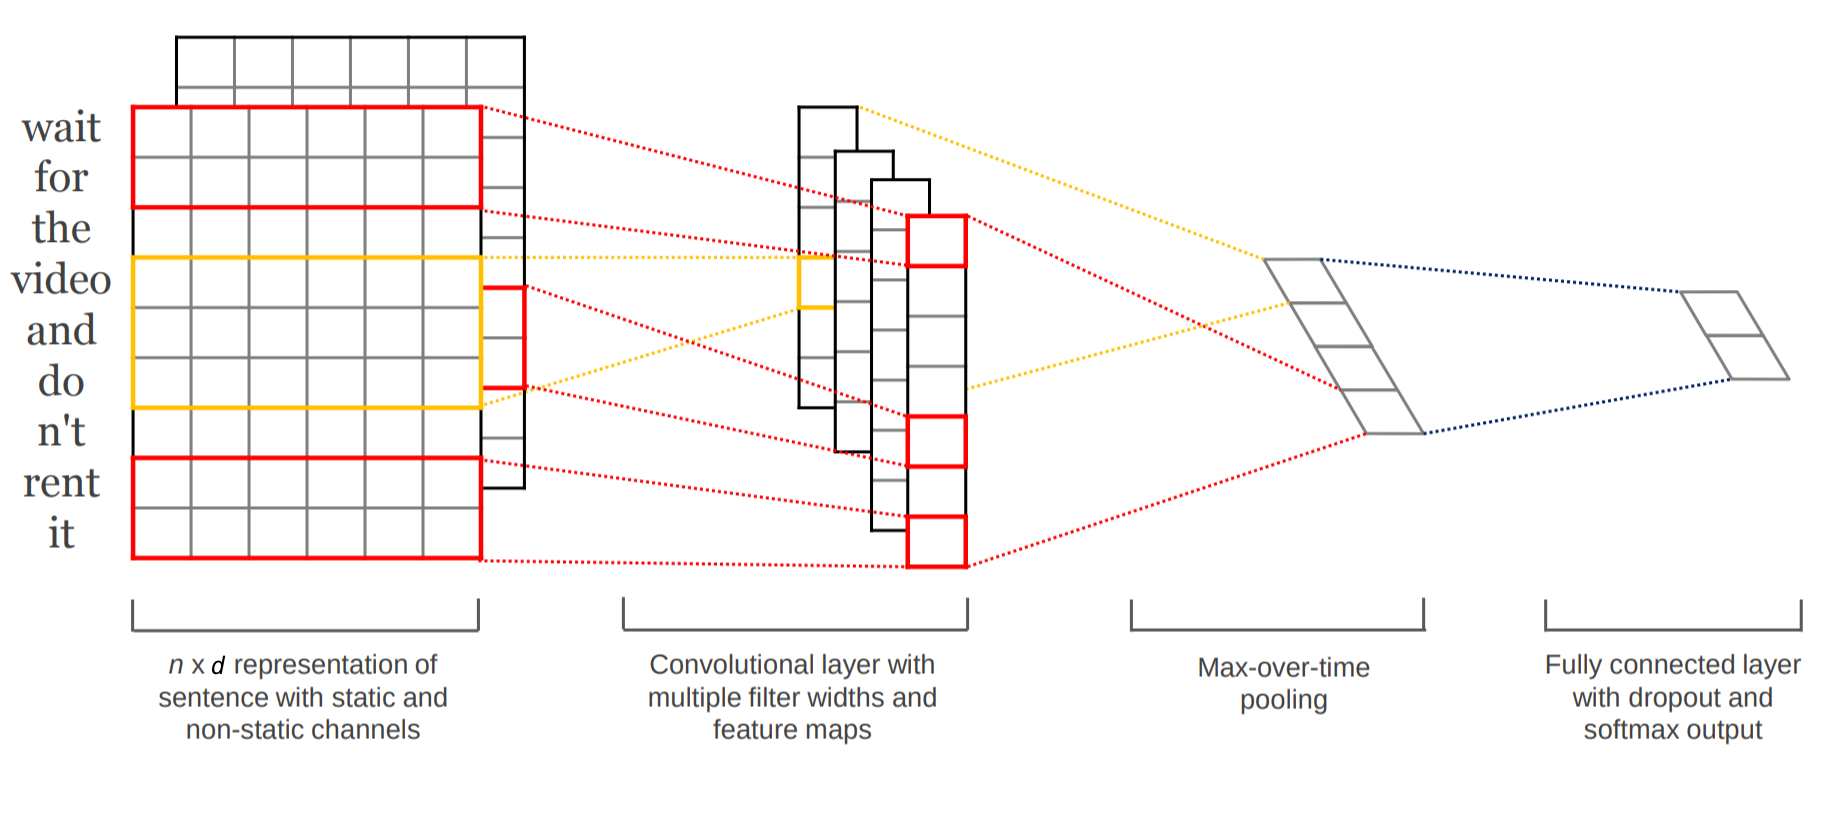
\includegraphics[width=70mm]{fig2.png}}
\caption{Convolutional Neural Network Architecture [2]}
\label{fig}
\end{figure}

\subsection{BERT}

Initially the authors employed a BERT tokenizer, pretrained on an uncased corpus, and utilized default settings. However, we quickly learned that classification with BERT default parameters yields predicting the majority class. With specific optimizer parameters and freezing a few layers, it allowed for the model to learn better than its default counterpart.

\begin{figure}[htbp]
\centerline{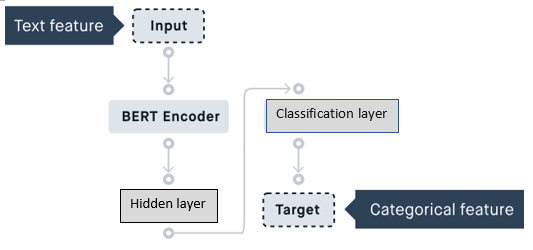
\includegraphics[width=70mm]{fig3.png}}
\caption{BERT Structure}
\label{fig}
\end{figure}

\section{Results}

\begin{table}[htbp]
\caption{Model Results}
\begin{center}
\begin{tabular}{|c|l|l|l|l|l|l|c|l|l|}
\hline
\multicolumn{7}{|c|}{\textbf{Models}}    & \multicolumn{3}{c|}{\textbf{Accuracy}} \\ \hline
\multicolumn{7}{|c|}{Tf-idf with Logistic Regression}  & \multicolumn{3}{c|}{84.85\%}     \\ \hline
\multicolumn{7}{|c|}{Tf-idf Feed-Forward Neural network} & \multicolumn{3}{c|}{95.08\%}     \\ \hline
\multicolumn{7}{|c|}{Word2Vec with CNN}   & \multicolumn{3}{c|}{98.04\%}     \\ \hline
\multicolumn{7}{|c|}{BERT}      & \multicolumn{3}{c|}{89.05\%}     \\ \hline
\end{tabular}
\label{tab1}
\end{center}
\end{table}

Tf-idf with Logistic Regression is too low to use as a model baseline; Tf-idf Feed-Forward Artificial Neural network is a good baseline as it accurately classifies a good portion of the data with room for improvement. With our own research Word2Vec with CNN performed the best with a test accuracy of 98.04\%. However, BERT on its own, did not perform as well as we had hoped with an accuracy lower than our baseline at 89.05\%. 


\section{Error Analysis}

\subsection{False Positive Tweets}
\begin{quotation}
\emph{RT @Juliet777777: Video Pat Condell “Nothing to do with Islam” The death rattle of a dhimmi society..}
\end{quotation}
\begin{quotation}
\emph{@Lithobolos @PoliticalAnt @ZaibatsuNews Christianity is dying.  Less attendance all the time. Total liberalization of the religion.}
\end{quotation}
\begin{quotation}
\emph{RT @adriarichards: With so many factual errors @NYTimes piece about online harassment by @jonronson, it's a disservice to everyone.}
\end{quotation}

Most false positive tweets contain words with negative sentiment and display emotionally charged words without specifically attacking any individual or group.

\subsection{False Negative Tweets}
\begin{quotation}
\emph{Kat's not a morning person. Or a midday person. Or an afternoon person. Or an evening person. Wait. Is she even a person??  \#mkr \#MKR2015}
\end{quotation}
\begin{quotation}
\emph{RT @itsbariecool @Mccheesy904 it happens vice versa but men are smarter naturally \#NotSexist}
\end{quotation}
\begin{quotation}
\emph{Maybe the girls should have less tickets on themselves and worry about the cooking. \#MKR}
\end{quotation}

Most false negative tweets employ an underlying tone of sarcasm and surprisingly a good amount of them contain hashtags like \#mkr; which may represent some form of unique sarcastic sentiment. False negative tweets may be more difficult to classify due to hidden meanings and less direct forms of attack. Also, some bullying tweets contains hashtag like \#notSexist or \#notRacist, which makes it harder for the model to discern them with actual neutral tweets. More examples of such attacks may be needed for an algorithm to detect such outliers.

\section{Conclusion}

Word2Vec with CNN performed the best as the training and test accuracies are above 98\%. With little room for improvement, no amount of optimizations will be able to increase training and test accuracies and error analysis indicates that improvements will require targeting of specific tweets; our NLP models are not able to detect such outliers.
	Cyberbullying will not be completely eliminated as it evolves and rears its head in different forms. Though our model correctly classified 98\% of tweets, we are still very concerned about our type II error rate as the impact of an unprevented cyberbullying tweet is immense. With 4.66 billion internet users, if 1\% of this population were to receive a cyberbullying message, that would be tremendous. For global communications platforms, a sentiment analysis model with an error rate of <1\% is essential to preserving a safe community. CNN along with feature extraction methods and a word embedding feature superior to Word2Vec would potentially be a more successful candidate for model improvement. One possible combination would be to utilize BERT with CNN.


\begin{thebibliography}{00}
\bibitem{b1} Huang, Qianjia, et al. “Cyberbullying Intervention Based on Convolutional Neural Networks.” ACL Anthology, Association for Computational Linguistics, Aug. 2018.
\bibitem{b2} Yoon Kim, Convolutional Neural Networks for Sentence Classification. New York University, 2014.
\end{thebibliography}

\end{document}
